% Chapter Template

\chapter{Evaluation of VAD algorithms} % Main chapter title

\label{Chapter3} % Change X to a consecutive number; for referencing this chapter elsewhere, use \ref{ChapterX}

\lhead{Chapter 3. \emph{Evaluation of VAD algorithms}} % Change X to a consecutive number; this is for the header on each page - perhaps a shortened title

%----------------------------------------------------------------------------------------
%	SECTION 1 - 
%----------------------------------------------------------------------------------------

\section{Evaluation methods}

Voice Activity Detection is a binary classification problem for which a number of standard evaluation methods are typically used.

\section{Implementation details}

\subsection{Selected VAD algorithms and their parameters}

\subsection{Hang-over scheme}

\subsection{Speech recordings}

\subsection{Noise types and SNR}

\section{Evaluation results}

\begin{figure}[htbp]
	\centering
		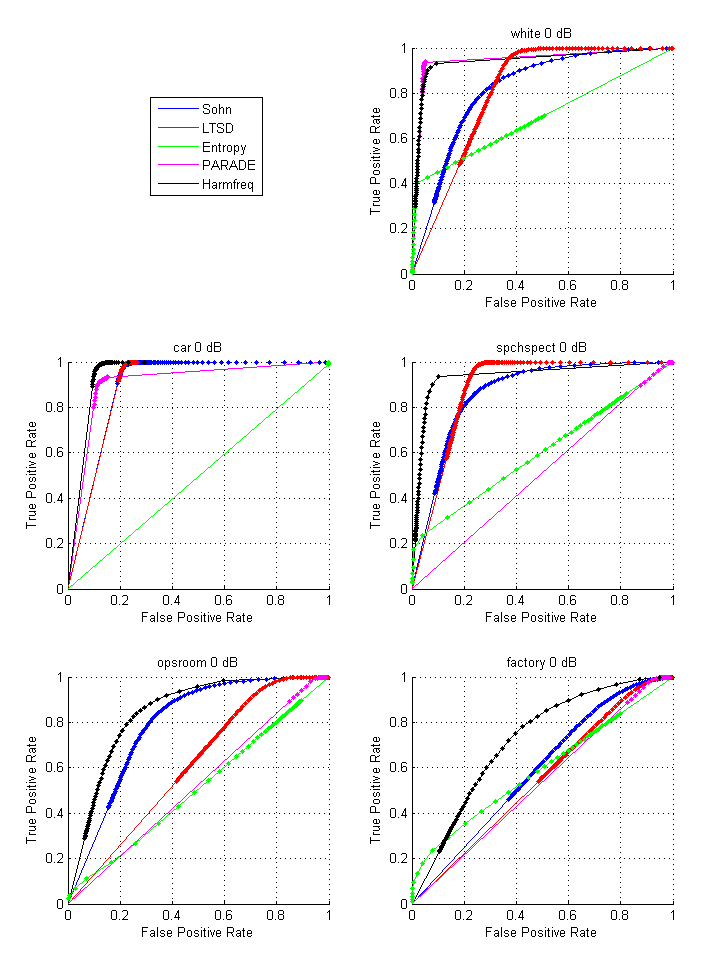
\includegraphics[width=1.0\columnwidth]{Figures/Chapter3/0dB.png}
		\rule{37em}{0.5pt}
	\caption[ROC curves of the evaluated VAD algorithms under 0 dB SNR]{ROC curves of the evaluated VAD algorithms under 0 dB SNR}
	\label{fig:0dB}
\end{figure}

\begin{figure}[htbp]
	\centering
		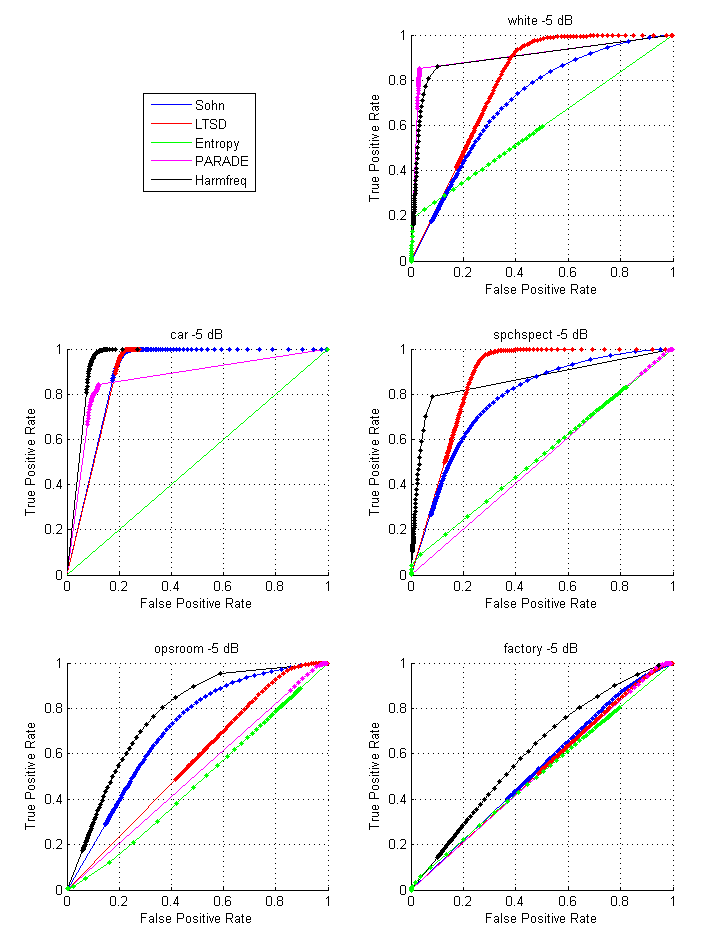
\includegraphics[width=1.0\columnwidth]{Figures/Chapter3/-5dB.png}
		\rule{37em}{0.5pt}
	\caption[ROC curves of the evaluated VAD algorithms under -5 dB SNR]{ROC curves of the evaluated VAD algorithms under -5 dB SNR}
	\label{fig:-5dB}
\end{figure}

\begin{table}[htbp]
\center
\begin{tabular}{c|c|c|c|c|c|}
\cline{2-6}
 & Sohn & LTSD & Entropy & PARADE & Harmfreq \\ \hline
\multicolumn{1}{ |c| }{white} & 0.8176 & 0.8083 & 0.6921 & \textbf{0.9484} & 0.9415 \\ \hline
\multicolumn{1}{ |c| }{car} & 0.8948 & 0.8939 & 0.4942 & 0.9075 & \textbf{0.9471} \\ \hline
\multicolumn{1}{ |c| }{spchspect} & 0.8617 & 0.8829 & 0.6018 & 0.5100 & \textbf{0.9367} \\ \hline
\multicolumn{1}{ |c| }{opsroom} & 0.7906 & 0.6131 & 0.5103 & 0.5243 & \textbf{0.8447} \\ \hline
\multicolumn{1}{ |c| }{factory} & 0.5889 & 0.5503 & 0.5909 & 0.5351 & \textbf{0.7197} \\ \hline
\end{tabular}
\caption[AUC values of the evaluated VAD algorithms under 0 dB SNR]{AUC values of the evaluated VAD algorithms under 0 dB SNR}
\label{tab:AUC0dB}
\end{table}

\begin{table}[htbp]
\center
\begin{tabular}{c|c|c|c|c|c|}
\cline{2-6}
 & Sohn & LTSD & Entropy & PARADE & Harmfreq \\ \hline
\multicolumn{1}{ |c| }{white} & 0.7088 & 0.7851 & 0.5919 & \textbf{0.9104} & 0.8999 \\ \hline
\multicolumn{1}{ |c| }{car} & 0.8971 & 0.8960 & 0.4999 & 0.8692 & \textbf{0.9520} \\ \hline
\multicolumn{1}{ |c| }{spchspect} & 0.7811 & 0.8660 & 0.5274 & 0.5060 & \textbf{0.8643} \\ \hline
\multicolumn{1}{ |c| }{opsroom} & 0.7040 & 0.5705 & 0.4741 & 0.5144 & \textbf{0.7716} \\ \hline
\multicolumn{1}{ |c| }{factory} & 0.5378 & 0.5265 & 0.5150 & 0.5212 & \textbf{0.6084} \\ \hline
\end{tabular}
\caption[AUC values of the evaluated VAD algorithms under -5 dB SNR]{AUC values of the evaluated VAD algorithms under -5 dB SNR}
\label{tab:AUC-5dB}
\end{table}

\section{Conclusion}